\documentclass[tikz,border=2pt]{standalone}
\usepackage{amsmath}
\usepackage{amssymb}
\usepackage{xcolor}

\definecolor{journalink}{HTML}{1F1C18}
\definecolor{journalmuted}{HTML}{8A7F72}
\definecolor{journalaccent}{HTML}{9C2D2D}

\begin{document}
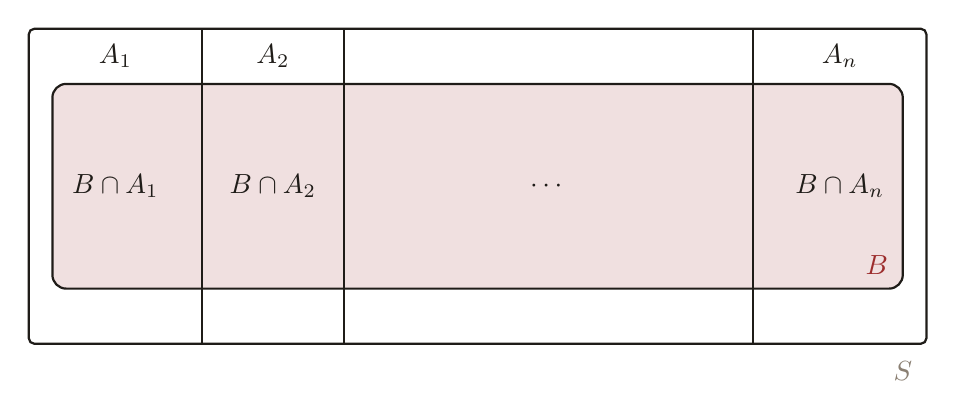
\begin{tikzpicture}[
  x=1cm,
  y=1cm,
  every node/.style={font=\normalsize}
]
  \fill[journalaccent, fill opacity=0.15, rounded corners=5pt]
    (-5.4,-1.3) rectangle (5.4,1.3);

  \draw[journalink, line width=0.8pt, rounded corners=2pt]
    (-5.7,-2) rectangle (5.7,2);

  \draw[journalink, line width=0.8pt] (-3.5,-2) -- (-3.5,2);
  \draw[journalink, line width=0.8pt] (-1.7,-2) -- (-1.7,2);
  \draw[journalink, line width=0.8pt] (3.5,-2) -- (3.5,2);

  \draw[journalink, line width=0.8pt, rounded corners=5pt]
    (-5.4,-1.3) rectangle (5.4,1.3);

  \node[journalink] at (-4.6,1.65) {$A_1$};
  \node[journalink] at (-2.6,1.65) {$A_2$};
  \node[journalink] at (4.6,1.65) {$A_n$};

  \node[journalink] at (-4.6,0) {$B\cap A_1$};
  \node[journalink] at (-2.6,0) {$B\cap A_2$};
  \node[journalink] at (0.9,0) {$\cdots$};
  \node[journalink] at (4.6,0) {$B\cap A_n$};

  \node[journalaccent] at (5.07,-1) {$B$};
  \node[journalmuted] at (5.4,-2.35) {$S$};
\end{tikzpicture}
\end{document}
